\chapter{USB}
USB ist eine Schnittstelle, welche so gut wie alle mordernen Rechner bsitzten. Es ist unter anderem Möglich darüber Geräte wie Kopfhörer, Joysticks aber auch Wechseldatenträger an zu schließen. Im letzteren Bereich ersetzt USB die bisher vorherschende CD/DVD-Technologier, da auf einem USB Stick mehr Daten in höherer Geschwindigkeit gespeichert werden können.
\section{Gefahren bei USB}\label{GefBeiUSB}
USB-Geräte stellen Gefahren auf verschiedenen Ebenen dar. Zum einen werden USB-Sticks, zumindest in dem Szenario, das hier betrachtet wurde, von Dritten an Mitarbeiter gegeben. Das heist, dass der Dritte, insofern dieser die nötige kriminielle Energie aufweist, ein prepariertes Gerät einschicken könnte. Erschwerend kommt hinzu, dass der Mitarbeiter keine Möglichkeit hat, ein böses USB-Gerät von einem normalen zu unterscheiden. Auch besteht die Möglichkeit für den Dritten den Angriff über längerere Zeit vorzubereiten, da kein Zeitdruck besteht, im Gegenteil, USB-Geräte sind gerade noch im Aufwärtstrend. TODO CD vs USB Statistik. Bei der Manipulation sind verschiedene Szenarien denkbar. Einige sind in den nächsten Sektionen aufgeführt.

\subsection{Viren}
Viren sind eine wachsende Bedrohung in der heutigen Zeit. Vor einigen Jahren waren einige wenige Virenfamilien weit verbreitet. So konnten Virenhersteller über signaturbasierte Suchalgorithmen nach bekannten Mustern suchen und Viren identifizieren. In den letzten Jahren zeichnet sich jedoch der Trend ab, dass Viren sich schneller weiterentwickeln und zudem oft polymorph programmiert sind, also ihr aussehen bei einer Infektion verändern. Dadurch werden signaturbasierte Erkennungen immer uneffizienter und die Gefahr, dass ein Rechner unerkannt Infiziert wird, steigt. Eine Infektion passiert zumeist über sogenannte Browserexploits, also preparierte Webseiten, welche Lücken in der Software des Users nutzten, oder durch E-Mails verbreitet. In dem von uns betrachteten Szenario würde ein krimineller Dritter oder aber auch ein unwissinder Dritter, dessen Rechner von einem Virus infiziert ist, einen USB-Stick mit einem Virus einschicken. Dabei wird im folgenden zwischen Trojaner, welche sich auf der Treiberebene einnissten, unterschieden.

\subsubsection{Viren auf Dateiebene}
Ein Trojaner ist eine Programm, welches sich als normale Software tarnt aber Schadcodefunktionalität mitliefert. \cite{Stamp2006} Will ein Benutzer das vermeitlich sinnvolle Programm installieren, wird im Hintergrund unbemerkt die Schadroutine mitinstalliert und gestartet. Dieser Schadecode hat oftmals Funktionalitäten wie Keylogger, Backdoors oder ein herkömmliches Rootkit. Auf unser Szenario übertragen müsste ein Benutzer also einen USB-Stick einstecken und ein darauf befindliches Programm starten. Ist der Virus bereits bekannt, könnte Virenscanner diesen finden un blockieren, jedoch ist es Aufgrund des Fortschritts immer öfter der Fall, dass Viren sich trotz gleicher Funktionaliät ihr aussehn veränder und dadruch von den Pattern des Virenschutzes nicht mehr erfasst werden.
			
\subsubsection{Viren auf Treiberebene}
Schwieriger zu entdecken sind Viren auf Treiberebene. Diese Nutzen lücken in der Firmware der im Computer verbauten Hardware und infizieren diese. So zeigte Karsten Nohl TODO Quelle zuletzt einen Angriff, in welchem er einen USB-Stick so manipuliert, dass dieser bei Kontakt mit einem Computer einen entsprechenden Trojaner ausführt. Dieser Trojaner war jedoch wiederrum in der Lange, andere USB-Stickts zu infizieren.

\subsection{Dateneinschleußung}

			
\subsection{Datenabfluss}
Neben den Gefahren von außen müssen jedoch auch sogenannte \glqq Inside-Threaths\grqq beachtet werden. Dies wären Mitarbeiter, welche z.B. interne IT-Systeme manipulieren, um sich Vorteile oder Reichtümer zu verschaffen. Das wohl bekannteste Beispiel wäre hier wohl ein TODO Kevin Midnick Geschichte. Bezogen auf USB wäre ein Risiko der Abfluss von Daten, also wenn ein Mitarbeiter Daten auf einem USB-Stick speichert und diese mit nach Hause nimmt, um diese zu Verkaufen oder sich zu bereichern. Denkbar wären zum Beispiel Kundendaten, bei Admins Passwörter, Geschäftsberichte oder sonstige Unternehmensgeheimnisse. Diese können oft für Geld in einschlägigen Bereichen des Internets verkauft oder bei Geschäftsberichten zur Manipulation am Finanzmarkt genutzt werden. Auch wäre eine Abwerbung eines Mitarbeiters von einem anderen Unternehmen für Industriespionage denkbar.
Eine neue Bedrohung sind Geheimdienste, welche Personen in eine Unternehmen einschleußen oder Mitarbeiter abwerben, um Daten übe die Kunden zu sammeln. Dies wurde erst letztens durch von Edward Snowden veröffentlichte Dokumente publik. TODO Quelle

\section{Technische Ablauf beim Einstecken eines USB-Devices}
Einstecken => Felder werden übertragen => Windows sucht nach Treiber und installiert diese

\section{Descriptoren}
Der USB-Specifikation, welche von dem USB Implementers Forum, Inc.\footnote{http://www.usb.org/about} festgelegt wird, sieht Felder vor, welche Informationen zu dem Gerät beinhalten.
\begin{wrapfigure}{l}{0pt}%{0.5\textwidth}
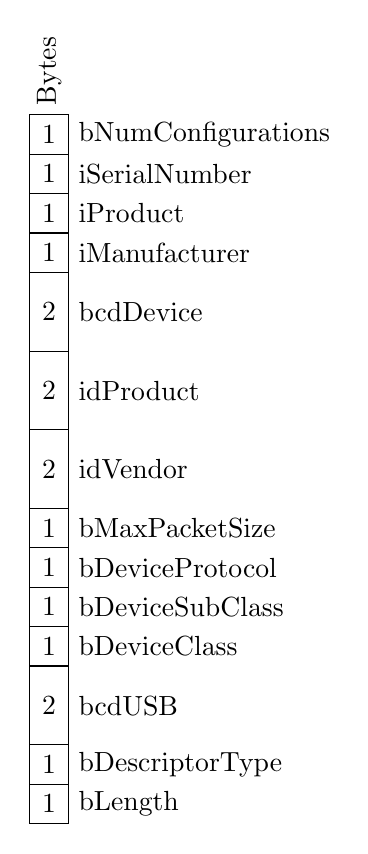
\begin{tikzpicture}[scale=1]
	\draw (0,0) rectangle (0.5,0.5);
	\draw (0.25, 0.25) node {1};
	\draw (0.5, 0.25) node[right]{bLength};
	
	\draw (0,0.5) rectangle (0.5,0.5);
	\draw (0.25, 0.75) node {1};
	\draw (0.5, 0.75) node[right]{bDescriptorType};
	
	\draw (0,1) rectangle (0.5,1);
	\draw (0.25,1.5) node {2};
	\draw (0.5,1.5) node[right]{bcdUSB};
	
	\draw (0,2) rectangle (0.5,0.5);
	\draw (0.25,2.25) node {1};
	\draw (0.5,2.25) node[right]{bDeviceClass};

	\draw (0,2.5) rectangle (0.5,0.5);
	\draw (0.25,2.75) node {1};
	\draw (0.5,2.75) node[right]{bDeviceSubClass};

	\draw (0,3) rectangle (0.5,0.5);
	\draw (0.25,3.25) node {1};
	\draw (0.5,3.25) node[right]{bDeviceProtocol};

	\draw (0,3.5) rectangle (0.5,0.5);
	\draw (0.25,3.75) node {1};
	\draw (0.5,3.75) node[right]{bMaxPacketSize};
	
	\draw (0,4) rectangle (0.5,1);
	\draw (0.25,4.5) node {2};
	\draw (0.5,4.5) node[right]{idVendor};
	
	\draw (0,5) rectangle (0.5,1);
	\draw (0.25,5.5) node {2};
	\draw (0.5,5.5) node[right]{idProduct};
	
	\draw (0,6) rectangle (0.5,1);
	\draw (0.25,6.5) node {2};
	\draw (0.5,6.5) node[right]{bcdDevice};
	
	\draw (0,7) rectangle (0.5,0.5);
	\draw (0.25,7.25) node {1};
	\draw (0.5,7.25) node[right]{iManufacturer};
	
	\draw (0,7.5) rectangle (0.5,0.5);
	\draw (0.25,7.75) node {1};
	\draw (0.5,7.75) node[right]{iProduct};
	
	\draw (0,8) rectangle (0.5,0.5);
	\draw (0.25,8.25) node {1};
	\draw (0.5,8.25) node[right]{iSerialNumber};
	
	
	\draw (0,8.5) rectangle (0.5,0.5);
	\draw (0.25,8.75) node {1};
	\draw (0.5,8.75) node[right]{bNumConfigurations};
	
	\draw (0,9) rectangle (0.5,0.5);
	
	\draw (0.25, 9) node[rotate=90, right] {Bytes};
\end{tikzpicture}
\caption{USB-Felder}
\end{wrapfigure}

Dies Umfasst die technische Informationen wie die Länge der gesamten Felder im \glqq bLength\grqq-Feld oder das Protokoll des Geräts im \glqq bDeviceProtocoll\grqq-Feld über Informationen für das Betriebssystem wie \glqq idVendor\grqq, \glqq idProduct\grqq, \glqq bDeviceSubClass\grqq und \glqq bDeviceClass\grqq. Diese Felder mit der jeweiligen Länge sind in der Grafik dargestellt. Ein Feld hat dabei zwischen ein und zwei Bytes. Die Felder \glqq bDeviceClass\grqq, \glqq bDeviceSubClass\grqq, \glqq bDeviceProtocol\grqq sowie \glqq idVendor\grqq werden vom Herrsteller befüllt.\footnote{http://www.beyondlogic.org/usbnutshell/usb5.shtml} Das Betriebssystem nutzt die Felder meist um Treiber zu suchen oder auch das angeschlossene USB-Gerät gegen die Policie-Einstellungen zu prüfen. Um eigene Werte bei PID oder VID-Felder zu nutzten und damit sicher gestellt ist, dass nicht mehrere Herrsteller die selbe PID verwenden, müssen die Addressbereiche der PID bei dem USB Implementers Forum, Inc. gekauft werden. Dazu gibt es zwei Möglichkeiten. Man kann entweder ein Mitglied werden, wobei kosten von 5000 USD jährlich anfallen oder einmalig 5000 USD für einen Adressraum zahlen, man darf dann jedoch nicht das offizielle USB-Logo verwenden. \footnote{http://www.usb.org/developers/vendor/} Im folgenden werden die für dieses Dokument interessanten Felder weiter erläutert:

%\begin{figure}[h]
%	\setlength{\unitlength}{0.14in} % selecting unit length
%	\centering % used for centering Figure
%	\begin{picture}(36,10) % picture environment with the size (dimensions)
%% 32 length units wide, and 15 units high.
%		\put(0,4){BlaBLab}
%		\put(0,0){\framebox(2,3){1}}
%		\put(2,0){\framebox(2,3){1}}
%		\put(4,0){\framebox(4,3){1}}
%		\put(8,0){\framebox(2,3){1}}
%		\put(10,0){\framebox(2,3){1}}
%		\put(12,0){\framebox(2,3){1}}
%		\put(14,0){\framebox(2,3){1}}
%		\put(16,0){\framebox(4,3){1}}
%		\put(20,0){\framebox(4,3){1}}
%		\put(24,0){\framebox(4,3){1}}
%		\put(28,0){\framebox(2,3){1}}
%		\put(30,0){\framebox(2,3){1}}
%		\put(32,0){\framebox(2,3){1}}
%		\put(34,0){\framebox(2,3){1}}
%		\put(23,4){\framebox(6,3){$H_{C}(q)$}}
%		\put(0,5.5){\vector(1,0){3}}
%		\put(19.5,6.5) {$x_{C}(k)$}
%	\end{picture}
%	\caption{Aufbau der USB-Descriptoren}
%	% title of the Figure
%	\label{fig:lnlblock}
%	% label to refer figure in text
%\end{figure}			
$ $\\ \\ \\ \\ \\
\begin{description}
	\item[idVendor: ] Das idVendor-Feld wird von der USB Implementers Forum, Inc. festgelegt. Das Feld ist 2 Byte lang und ein Wert ist genau einem Herrsteller zugeordnet. Ersteht ein Unternehmen eine idVendor-Nummer, kann er über das idProduct-Feld frei verfügen.
	\item[idProduct: ] Das idProduct-Feld wird von einem Unternehmen vergeben, welches einen Wert im idVendor-Feld gekauft hat. Es ist ebenfalls 2 Byte lang. Damit könnte ein Unternehmen bis zu $2^{16}$ verschiedene Produkte beschreiben.
	
\end{description}
Das Feld PID steht für Produkt \glqq Identifier\grqq und beschreibt den Herrsteller des Geräts. TODO Tabelle